% Created 2017-09-24 Sun 14:56
\documentclass[11pt]{article}
\usepackage[utf8]{inputenc}
\usepackage[T1]{fontenc}
\usepackage{fixltx2e}
\usepackage{graphicx}
\usepackage{longtable}
\usepackage{float}
\usepackage{wrapfig}
\usepackage{rotating}
\usepackage[normalem]{ulem}
\usepackage{amsmath}
\usepackage{textcomp}
\usepackage{marvosym}
\usepackage{wasysym}
\usepackage{amssymb}
\usepackage{hyperref}
\tolerance=1000
\date{Sept 25-29, 2017}
\title{Week 5 lecture notes - PSYC 3330}
\hypersetup{
  pdfkeywords={},
  pdfsubject={},
  pdfcreator={Emacs 25.2.1 (Org mode 8.2.10)}}
\begin{document}

\maketitle
So far this semester, we have used statistics to \textbf{describe} data.  Now, we will begin using statistics as an \textbf{inference tool}.  To do this, we need to discuss \textbf{probability}.

\section*{Definition}
\label{sec-1}

Suppose we have a list of possible \emph{outcomes}, labeled A, B, C, D, and so on.  Then:

\[
p(A) = \text{ "the probability of A" }=\frac{\text{number of outcomes classified as A}}{\text{total number of possible outcomes}}
\]

Example: What is the probability of picking a king of spades from a standard deck of 52 cards?

Answer:

\[
p(\text{king of spades}) = \frac{\text{# of times king of spades appears}}{\text{number of cards in the deck}} = \frac{1}{52}
\]

Example: What is the probability of picking a heart from a deck?

Answer:

\[
p(\text{heart}) = \frac{\text{# hearts in a deck}}{\text{number of cards in the deck}} = \frac{13}{52} =\frac{1}{4} = 0.25
\]

The more common way we will encounter probability is as part of a \emph{probability distribution}.

Example: Suppose we have 40 slips of paper, each labeled with one of the numbers 1,2,3,4,5.  Specifically, assume they are labeled with the following frequencies:

\begin{center}
\begin{tabular}{rrr}
X & f & p\\
\hline
5 & 2 & 0.05\\
4 & 10 & 0.25\\
3 & 16 & 0.40\\
2 & 8 & 0.20\\
1 & 4 & 0.10\\
\end{tabular}
\end{center}

Visually, this distribution looks like the following graph:

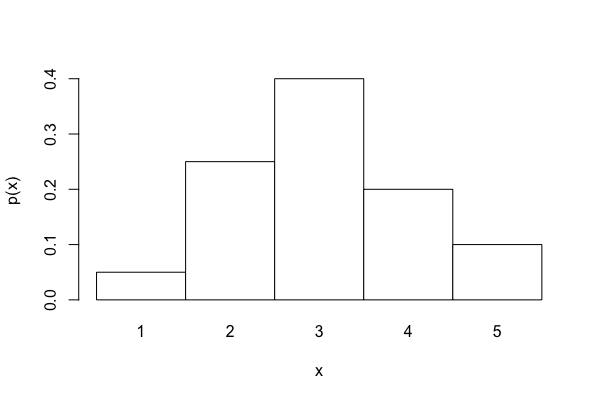
\includegraphics[width=.9\linewidth]{figures/week5/plot1.png}

Now, suppose our task is to randomly select a slip of paper.  We can then ask lots of questions, such as:

\begin{itemize}
\item What is the probability of selecting a 3?
\begin{itemize}
\item Answer: $p(3) = 0.40$
\end{itemize}
\item What is the probability of selecting a 5?
\begin{itemize}
\item Answer: $p(5) = 0.05$
\end{itemize}
\end{itemize}

We can also ask more complex questions:

\begin{itemize}
\item What is the probability of selecting a slip of paper with a value greater than 2?
\begin{itemize}
\item Answer: $p(x>2) = 0.40 + 0.25 + 0.05 = 0.70$
\end{itemize}
\end{itemize}

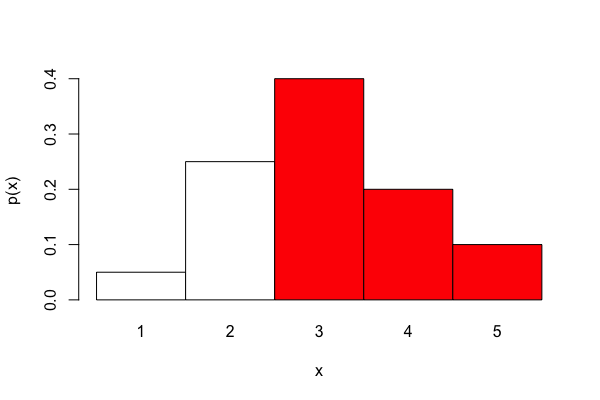
\includegraphics[width=.9\linewidth]{figures/week5/plot2.png}

\begin{itemize}
\item What is the probability of selecting a slip of paper with a value less than 5?
\begin{itemize}
\item Answer: $p(x<5) = 0.10 + 0.20 + 0.40 + 0.25 = 0.95$
\end{itemize}
\end{itemize}

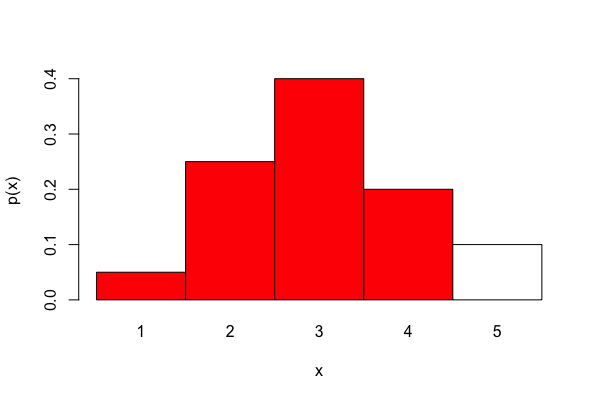
\includegraphics[width=.9\linewidth]{figures/week5/plot3.png}

\begin{itemize}
\item What is the probability of selecting a value greater than 1 and less than 4?
\begin{itemize}
\item Answer: $p(1 < x < 4) = 0.20 + 0.40 = 0.60$
\end{itemize}
\end{itemize}

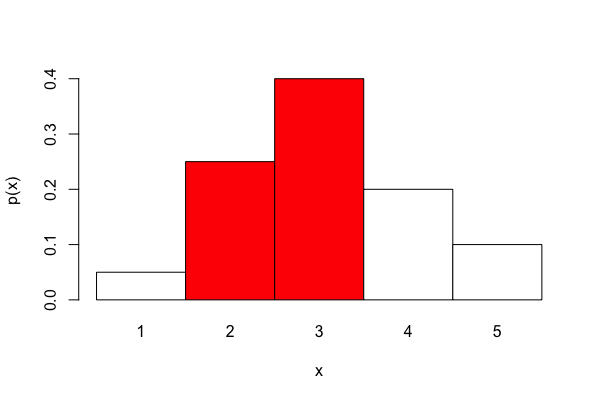
\includegraphics[width=.9\linewidth]{figures/week5/plot4.png}  
% Emacs 25.2.1 (Org mode 8.2.10)
\end{document}